\section{Problem Statement}

% \subsection{Motivation}

\begin{frame}
  \frametitle{Motivation}
  \begin{itemize}
    \item Protecting information in contested and congested wireless communication environments requires transmissions that are difficult to intercept or even detect (LPI/LPD). 
     \item Achieving robust protection against detection relies on signals with power spectral densities that are well below the noise floor. 
    % \item To recover the signals at low SNR, joint detection and carrier synchronization algorithms play a vital role in protected communication system. 
     \item At low SNR, the time and carrier synchronization are coupled problems:
     \begin{itemize}
      \item coherent methods for detecting signal require accurate carrier estimation, while
      \item data-aided carrier estimation requires the location of the training sequence.
     \end{itemize}
     \item In practice, the position of the embedded training sequence (preamble) should be searched sequentially.
     % explain using sliding window.
 \end{itemize}
\end{frame}

% \subsection{Previous Work}





\begin{frame}
    \frametitle{Research Contributions}
    % \begin{itemize}
    %     \item Our research provides a comprehensive treatment of the signal acquisition problem of protected communications, which basically includes
    %     \begin{itemize}
    %         \item a family of joint detection and estimation algorithm that emphasize computational complexity while maintaining near-optimal accuracy at very low SNR, and
    %         \item the implementation of the proposed algorithms on a standard SDR platform.
    %     \end{itemize} 
    % \end{itemize}

    % \begin{figure}
    %     \centering
    %     \begin{minipage}{.5\textwidth}
    %       \centering
    %       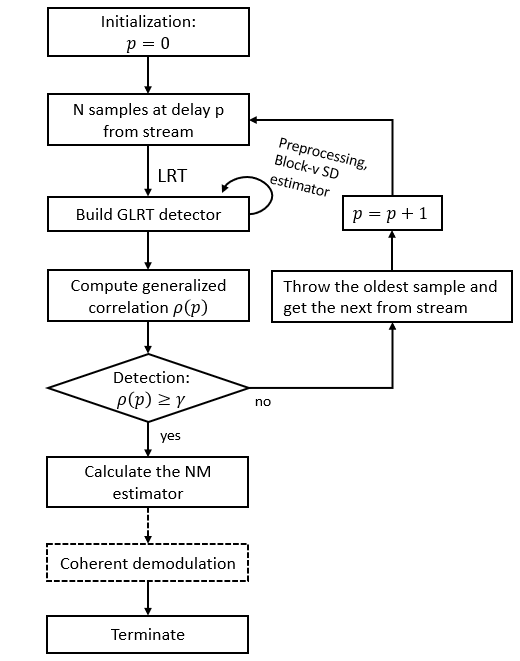
\includegraphics[width=.5\linewidth]{architecture_of_paper.png}
    %     \end{minipage}%
    %     \begin{minipage}{.5\textwidth}
    %       \centering
    %       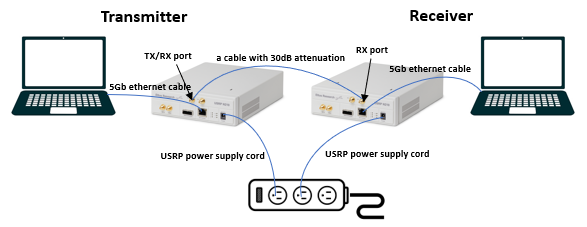
\includegraphics[width=.8\linewidth]{SDR_signal_transmission_path.png}
    %     \end{minipage}
    % \end{figure}
    \begin{columns}
      \begin{column}{0.54\textwidth}
        
        \begin{itemize}
          \item A comprehensive treatment of the signal acquisition problem of protected communications, which includes:      
          \begin{itemize}
              \item A family of joint detection and estimation algorithm:
              
              \begin{itemize}
                \item very low computational complexity, 
                \item near-optimal accuracy.
              \end{itemize}
              % that emphasize computational complexity while maintaining near-optimal accuracy at very low SNR, and
              \item Implementation of the proposed algorithms using a standard SDR platform.
          \end{itemize} 
        \end{itemize}

      \end{column} 

    \begin{column}{0.46\textwidth} 

        \begin{center}
          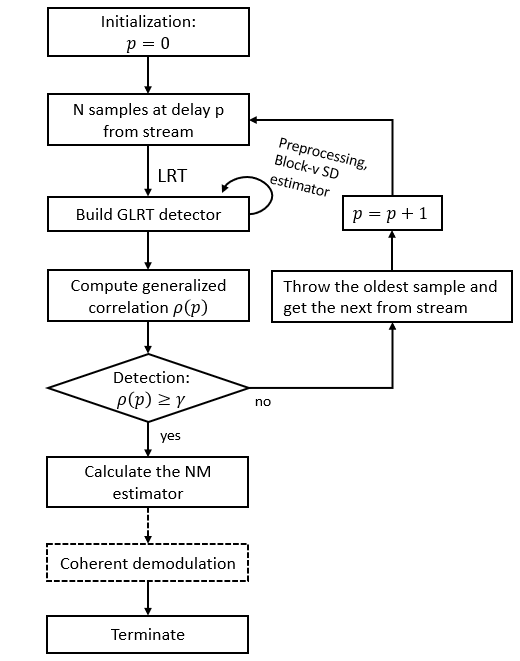
\includegraphics[width=.95\linewidth]{architecture_of_paper.png}
        \end{center}
      
      \end{column}
    \end{columns}

\end{frame}

\begin{frame}
  \frametitle{Prior Work}
  \begin{itemize}
      \item Some classical work on carrier synchronization assumes
        perfect time synchronization~\cite{Morelli_Mengali_98}. 
      \begin{itemize}
        \item  However, this is not reliable especially at low SNR.
      \end{itemize}
      \item Some  work on joint time and carrier synchronization
        problem shows good accuracy at low
        SNR~\cite{purushothaman_16,kim_17}.  
      \begin{itemize}
        \item Focus on frame synchronization instead of sequential detection, and 
        \item the complexity of the algorithm is relatively high.
      \end{itemize}
      \item Computational complexity is a major concern with the
        practical realization of a synchronization system discussed
        in~\cite{murin_16,wang_21}. 
  
  \end{itemize}
\end{frame}